\section{代数}
\subsection{十进制加减法}
任意的十进制数字可以写成\(\dis\sum_{n\in\Zs}^{}a_n10^n\)，其中\(a_n\in \{0\le a_n\le9 \left| a_n\in\Zs\right.\}\)

设任意两个整数\(\dis a = \sum_{n\in\Zs}^{}a_n10^n, b = \sum_{n\in\Zs}^{}b_n10^n\)，令\(\dis c = a + b = \sum_{n\in\Zs}^{}c_n10^n\)，其中\(
a_n, b_n\)都是小于\(10\)的非负整数，那么当\(i\in\Zs\)时，\(c_i = a_i + b_i\)，当\(c_i \ge 10\)时，令\(c_i = 10 + s\)，带入\(10^nc_i = 10^{n+1} + 10^ns\)，可以看出，\(c_{i+1}\)加了\(1\).
这个解释了加法的进一的原因。

设\(\dis d = a - b = \sum_{n\in\Zs}^{}d_n10^n\)，\(d_i = a_i - b_i\)，当\(d_i<0\)时，
令\(d_i = a_i + 10 - b_i\)，即借一位给第 \(i\) 位，同时 \(d_{i+1}\) 减 \(1\)。这解释了减法借位的原因。

\subsection{基本不等式}
我们都知道基本不等式\(\dis \frac{a+b}{2}\ge\sqrt{ab},a\ge0, b\ge0\)，当且仅当\(a=b\)时取等号。
\begin{proof}\itshape
\[
    (\sqrt{a}-\sqrt{b})^2=a+b-2\sqrt{ab}\ge0 \Rightarrow \frac{a+b}{2}\ge \sqrt{ab}
\]
可以看出当且仅当\(a = b\)时取等号.
\begin{figure}[H]
    \centering
    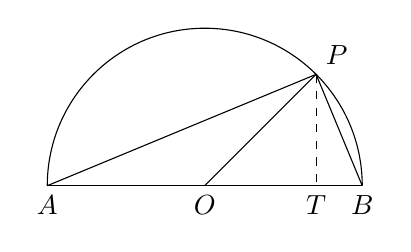
\begin{tikzpicture}
        \draw(2,0) arc(0:180:2);
        \draw(-2, 0)node[below]{\(A\)}--(2, 0)node[below]{\(B\)};
        \node[below] at(0,0){\(O\)};
        \draw(0, 0) --(45:2) node[above right]{\(P\)};
        \draw(2,0)--(45:2)--(-2,0);
        \draw[dashed](45:2)--(45:2|-0,0)node[below]{\(T\)};
    \end{tikzpicture}
    \caption{均值不等式的几何证明}
    \label{fig:basic-ineq-proof}
\end{figure}

如上图所示，\(\odot O, AB\perp PT, AT\cdot TB = (OP+OT)(OP-OT) = OP^2-OT^2 = PT^2\)，即
\(\dis \sqrt{AT\cdot TB} = PT\le \frac{AT + TB}{2} = OP\)
\end{proof}

\subsection{群论}
设非空集合\(S\)，上的二元运算\(\circ\)，满足下列条件：
\begin{itemize}
    \item 对于\(\forall a, b\in S\)，都满足\(a\circ b = c\in S\)；
    \item 对于\(\forall a, b, c\in S\)，都满足\((a\circ b)\circ c = a\circ(b\circ c)\)；
    \item 存在单位元，即幺元:\(e\in S\).对于\(\forall a\in S\)，都有\(e \circ a = a\)；
    \item 每个元素\(a\)都存在逆元素\(a^{-1}\in S\).有\(a^{-1}\circ a = e\)
\end{itemize}

的，把\(G(S, \circ)\)称为\textbf{群}。\textbf{群不一定满足交换律}，即可能\(a\circ b \ne b \circ a\).满足交换律的群称为交换群，也叫\textbf{阿贝尔群}。

下面证明群的单位元是唯一的，即\(e_l = e_r\)
\begin{proof}
    设 \(e_l\) 为左单位元，\(e_r\) 为右单位元，则
    \[
    e_l = e_l \circ e_r = e_r
    \]
    所以左单位元与右单位元相等，单位元唯一。
\end{proof}

下面证明每个元素的逆元是唯一的
\begin{proof}
    设 \(x, y\) 都是 \(a\) 的逆元，则：
    \[
    x = e \circ x = (y \circ a) \circ x = y \circ (a \circ x) = y \circ e = y
    \]
    所以逆元唯一。
\end{proof}


\subsection{复数}

虚数单位\(\mathrm{i}\)，即\(\mathrm{i}^2=-1\)，是方程\(x^2+1=0\)其中一个解.

所有的复数（\(\Cs\)）都可以表示成\(z=a+b\mathrm{i}\)的形式，其中\(a\)为复数\(z\)的实部，
记作\(a = \mathrm{Re}\ z\).\ \(b\)为虚部，记作\(b=\mathrm{Im}\ z\)，其中\(\overline{z}=a-b\mathrm{i}\)表示复数\(z\)的共轭复数。
\begin{figure}[H]
    \centering
    \begin{tikzpicture}
        \draw[->] (-2, 0)--(0,0) node[below left]{\(O\)}--(2, 0)node[below]{\(x\)};
        \draw[->](0, -2)--(0, 2) node[right]{\(y\)};
        \draw[->>](0, 0)--(1.5, 1) node[above]{\(Z(a, b)\)};
        \draw[dashed](1.5, 1)--(1.5, 0)node[below]{\(a\)};
        \draw[dashed](1.5, 1)--(0, 1)node[left]{\(b\)};
    \end{tikzpicture}
    \caption{复数\(z\)}
    \label{fig:complex-plane}
\end{figure}

如上图所示，在平面直角坐标系$xOy$中，\(Z(a, b)\)可以表示复数\(z = a + b\mathrm{i}\)，\(OZ^2 = a^2+b^2 = z\overline{z}\).当然，也可以用极坐标系来表示，形如\(z = R(\cos\theta + \mathrm{i}\sin\theta)\)

复数的加减运算
\begin{itemize}
    \item \(z_1 + z_2 = (a+b\mathrm{i}) + (c + d\mathrm{i}) = (a+c)+(b+d)\mathrm{i}\)
    \item \(z_1 - z_2 = (a+b\mathrm{i}) - (c + d\mathrm{i}) = (a-c)+(b-d)\mathrm{i}\)
\end{itemize}

下面讨论复数的乘除法

\begin{itemize}
    \item \(z_1z_2=r_1r_2(\cos(\theta_1+\theta_2) + \mathrm{i}\sin(\theta_1+\theta_2))\)
    \item \(\dis \frac{z_1}{z_2} = \frac{r_1}{r_2}(\cos(\theta_1-\theta_2) + \mathrm{i}\sin(\theta_1-\theta_2))\)
\end{itemize}

可以得出\(\dis |z_1z_2| = |z_1||z_2|,\ \left|\frac{z_1}{z_2}\right| = \frac{|z_1|}{|z_2|}\)

